\subsection{Audio, PWM}\label{sec:audioPWM}

Um ein Audiosignal abspielen zu können, werden zwei PWM-Signale benötigt wie in Abbildung \ref{fig:pwm_ausgang} ersichtlich. Das eine Signal ist die invertierte Variante des anderen Signals. 
Das PWM-Signal wird mit dem NRF52 generiert. Für den NRF52 stellt NORDIC SEMICONDUCTOR die PWM HAL and driver Bibliothek zur Verfügung. Die genutzten Funktionen sind in der Tabelle \ref{table:bibliothek} aufgeführt. Diese ermöglicht es, ein PWM-Signal zu erzeugen. Der NRF52 bietet vier PWM Instanzen mit je vier Kanälen. Für die Audioausgabe wurden zwei PWM Instanzen mit je einem Kanal genutzt.

\begin{table}[H]
	\centering
	\begin{tabular}{|l|l|l|}
		\hline
		%\rowcolor[HTML]{C0C0C0} 
		\textbf{Beschreibung} & \textbf{Funktion}                & \textbf{Argumente}                                                                                                                                                                                                            \\ \hline
		PWM initialisiern     & nrf\_drv\_pwm\_init              & \begin{tabular}[c]{@{}l@{}}nrf\_drv\_pwm\_t const *const p\_instance\\ nrf\_drv\_pwm\_config\_tconst *p\_config\\ nrf\_drv\_pwm\_handler\_thandler\end{tabular}                                                               \\ \hline
		Audio abspielen         & nrf\_drv\_pwm\_complex\_playback & \begin{tabular}[c]{@{}l@{}}nrf\_drv\_pwm\_t const *const p\_instance\\ nrf\_pwm\_sequence\_t const *p\_sequence\_0\\ nrf\_pwm\_sequence\_tconst *p\_sequence\_1\\ uint16\_t  playback\_count \\ uint32\_t  flags\end{tabular} \\ \hline
	\end{tabular}
	\label{table:bibliothek}
	\caption{Funktionen der PWM HAL and driver Bibliothek}
\end{table}

\begin{figure}[H]
	\begin{center}
		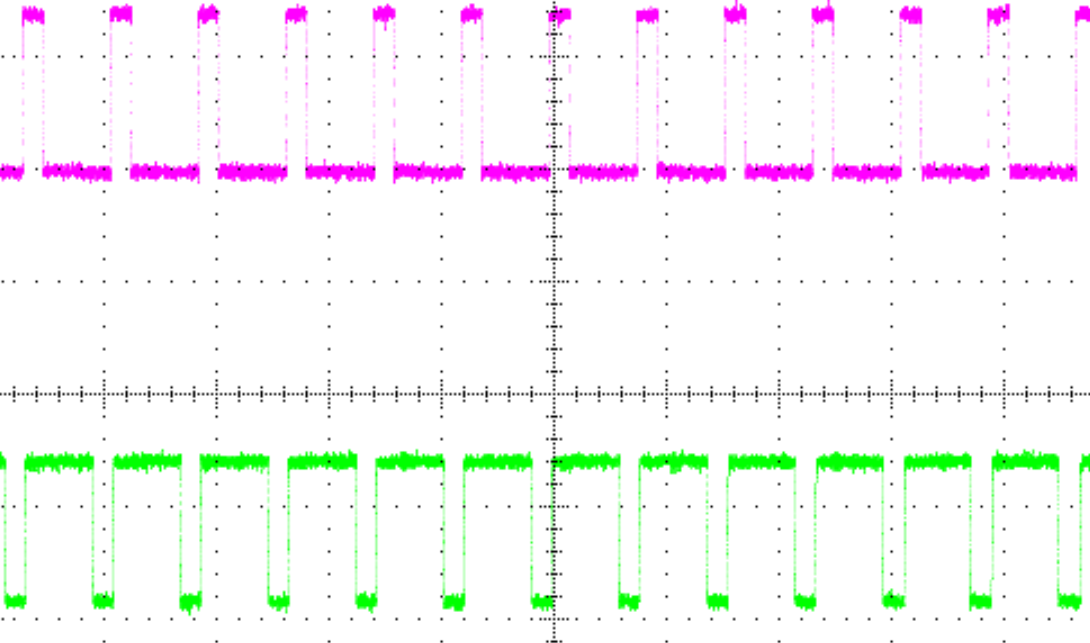
\includegraphics[width=80mm]{data/PWM_Signal_500Hz_Mono}
		\caption[PWM-Ausgang des NRF52]{PWM-Ausgang des NRF52. Das violette Signal ist das invertiere grüne Signal.} %picture caption
		\label{fig:pwm_ausgang}
	\end{center}
\end{figure}

In der Abbildung \ref{fig:pwm_ablauf} ist der Ablauf des PWM-Unterprogramm aufgezeigt. Als erstes findet die Initialisierung statt. Nach der Initialisierung können die beiden Sequenzen 0 und 1 generiert werden. In diesen Sequenzen sind die Daten des Audio-Files abgelegt. Die Funktion complex\_playback generiert am Ausgang anhand dieser Sequenzen das PWM-Signal.

\begin{figure}[H]
	\begin{center}
		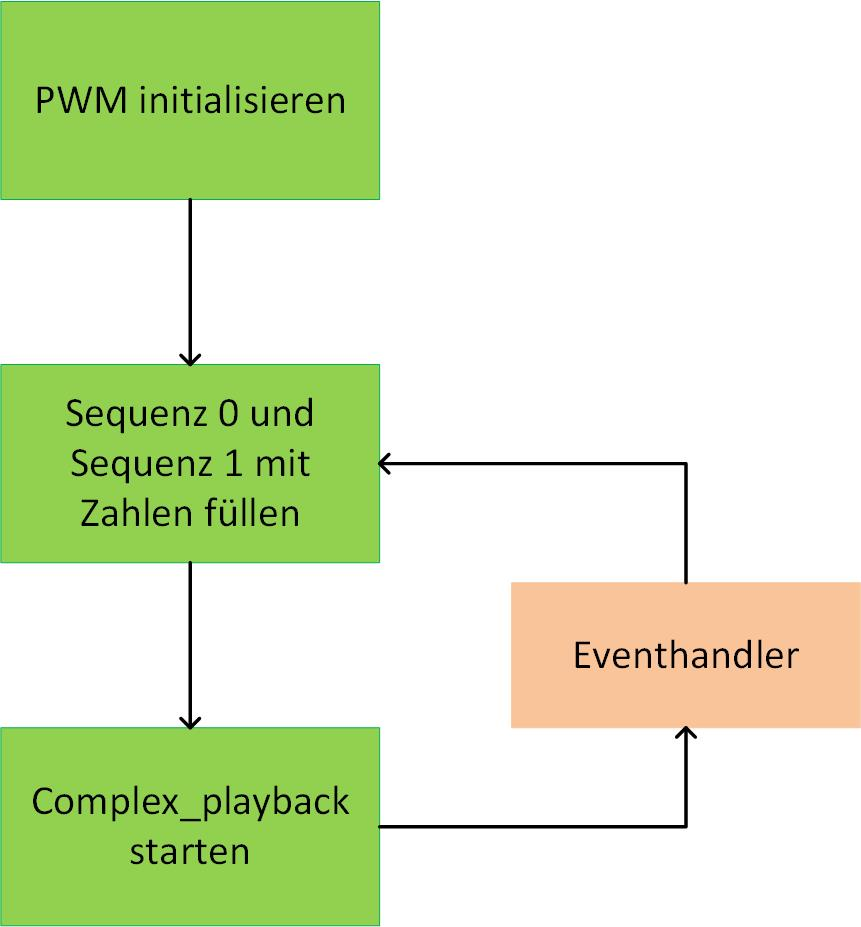
\includegraphics[width=60mm]{data/pwm_ablauf}
		\caption[Ablauf PWM]{Ablauf PWM} %picture caption
		\label{fig:pwm_ablauf}
	\end{center}
\end{figure}

\subsubsection*{PWM Initialisieren}\label{sec:PWM initialisieren}
Bei der Initialisierung wurde die PWM Instanz, die Config und der Eventhandler mitgegeben.  Die Config des PWM musste anhand der Angaben des Wavefiles generiert werden. Die Werte wurden wie in der Tabelle \ref{table:config} gewählt.

<<<<<<< HEAD
\begin{table}[H]
	\centering
	\begin{tabular}{|l|l|l|}
	\hline
	\textbf{Parameter}  & \textbf{Gewählter Wert}    & \textbf{Bemerkung}                                                           \\ \hline
	output\_pins  & Pin                        &                                                                              \\ \hline
	irq\_priority & APP\_IRQ\_PRIORITY\_LOWEST & Wurde aus dem Beispiel übernommen                                            \\ \hline
	base\_clock   & NRF\_PWM\_CLK\_16MHz       & Es wurde der höchste clock Frequenz gewählt                                  \\ \hline
	count\_mode   & NRF\_PWM\_MODE\_UP         & Wurde aus dem Beispiel übernommen                                            \\ \hline
	top\_value    & 500                        & Siehe Berechnung top Value                                                            \\ \hline
	load\_mode    & NRF\_PWM\_LOAD\_COMMON     & \begin{tabular}[c]{@{}l@{}}Wurde gewählt, da alle PWM Kanäle \\ den selben Wert ausgeben\end{tabular} \\ \hline
	stepp\_mode   & NRF\_PWM\_STEP\_AUTO       & Wurde aus dem Beispiel übernommen                                            \\ \hline
	\end{tabular}
	\caption{Gewählte Config Werte}
	\label{table:config}
\end{table}

\textbf{Berechnung top Value}\\
Da die clock Frequenz des PWM Moduls auf $16MHz$ gesetzt wurde, beträgt der top value für eine Audiodatei mit Abtastfrequenz von $32kHz 500$. Dies berechnet sich wie folgt:
=======
Da die clock Frequenz (oben *clock) des PWM Moduls auf $16MHz$ gesetzt wurde, beträgt der top value für eine Audiodatei mit Abtastfrequenz von $32kHz 500$. Dies berechnet sich wie folgt:
>>>>>>> bf25fa5cc30d7cbbed361af39edc0146dab9a6b3
\begin{equation}
32kHz = \frac{16MHz}{top \: value}
 \Rightarrow \; top \: value = \frac{16MHz}{32kHz} = 500
\end{equation}

\subsubsection*{Sequenzen laden}\label{sec:Sequenzen befüllen}
Mit der Funktion next\_Value werden neue Werte in die Sequenzen geladen. Diese Funktion ist im Abschnitt \ref{sec:sdKarte modul} genauer beschrieben.

\subsubsection*{Complex playback}\label{sec:Complex playback}
Die Funktion generiert anhand der Sequenz ein PWM-Signal. Der
Vorteil zu simple playback ist, dass zwei Sequenzen mitgegeben werden können. Wenn die Sequenz 0 fertig abgespielt wurde, startet automatisch die zweite Sequenz und der Eventhandler wird ausgelöst. In dieser Zeit kann die erste Sequenz wieder neu beladen werden. Die Beladung der Sequenzen wird mit dem Eventhandler dieser Funktion gesteuert. 
